\documentclass[12pt,a4paper]{report}

\usepackage[utf8]{inputenc}
\usepackage[english]{babel}
\usepackage[T1]{fontenc}
\usepackage{latexsym}
\usepackage{graphicx}
\usepackage{epsfig}
\usepackage{amsmath,amssymb,amsthm}
\usepackage[none]{hyphenat} 
\usepackage{float} % parametro H in figur : posizionamento esattamente li
\usepackage{verbatim}
\usepackage{booktabs}
\usepackage{enumerate} %lettere o altro negli indici
\usepackage{algorithmic} %float con un algoritmo
\usepackage[ruled]{algorithm} %[boxed]
\usepackage{subfig}    % + figure in un float figure
\usepackage{datetime}
\usepackage[rgb]{xcolor}
\usepackage{color} %testo colorato
\usepackage{tikz}
\usepackage{fullpage}
\usepackage{fancybox}

%con la classe book+openright lascio una pagina bianca a fine capitolo e dopo il titolo se necessario, con empty page queste pagine non sono numerate e non hanno stile
%%\usepackage{emptypage}


\usepackage{fancyhdr}
\setcounter{tocdepth}{3}

\frenchspacing
%\pagestyle{headings} % {headings,plain ,empty}
\linespread{1.3}
\DeclareGraphicsRule{.eps,.ps,.png}{bmp}{.bb}{} % formati utilizzabili con ordine di preferenza 
                                                % cosi non devo indicare le estensioni
\newcommand{\HRule}{\rule{\linewidth}{0.5mm}}

\newcommand{\algname}[1]{\ensuremath{\mbox{\sc #1}}}

\renewcommand{\algorithmicrequire}{\textbf{Input:}}
\renewcommand{\algorithmicensure}{\textbf{Output:}}
\renewcommand{\algorithmiccomment}[1]{// #1}
%\author{\emph{Marco Bettiol}\quad{} 586580\\\emph{Antonio Quercia}\quad{}  588537}

%per impaginare con giustifica sx-dx
  \tolerance 1414
  \hbadness 1414
  \emergencystretch 1.5em
  \hfuzz 0.3pt
  \widowpenalty=10000
  \vfuzz \hfuzz
  \raggedbottom

\title{}
\begin{document}
% !TEX root = tesi.tex
\begin{titlepage}

		\thispagestyle{empty}
    \begin{figure}
    \centering
      \subfloat{
\includegraphics[scale=1]{immagini/logo_unipd_black}}\quad     \subfloat{
\includegraphics[scale=1.3]{immagini/DEIlogoFULL}}
    \end{figure}
    
    \vskip 3cm{
    \begin{center}\sc
        UNIVERSITY OF PADUA\\
        DEPARTMENT OF INFORMATION ENGINEERING\\
        MASTER DEGREE IN COMPUTER ENGINEERING\end{center}
		}
		
		\vskip1.2cm\begin{center}
      \rm\large\uppercase\expandafter{A.A. 2009/2010\\}
 \end{center}
    	
    \vskip 2.5cm\begin{center}
    \HRule \\[0.4cm]\LARGE\expandafter{BATCH SIZE ESTIMATE}
    \HRule \\[0.4cm]
    \end{center}
    
    \begin{flushright}\vskip4.0cm 
    \begin{tabular}{rl}
            \rm\large \uppercase{Supervisor:} &\emph{Prof. Andrea Zanella}\\
	   \rm\large \uppercase{Student:} &\emph{Marco Bettiol} \\
		\end{tabular}
     \end{flushright}
    \vfill
          \begin{center}
                  \vskip1.0cm 
                  Last Update: \today  \hspace{1mm } \currenttime
           \end{center}
    
\end{titlepage}

\newpage
%%pagina vuota
%\clearpage\null\thispagestyle{empty}\clearpage

%\setcounter{page}{1}

\tableofcontents
%\listofalgorithms


\chapter{Introduction}

Generally speaking a set of actors contending for a common resource define a \emph{conflicting set}. As always, limited resources require policies to access them in an efficient and hopefully fair way. When the system is distributed, and this is our business, resource access can be assimilated to a coordination problem.\\ 
Physical medium access is our contended resource and several stations connect to the same physical medium to share it.\\ At the beginning of computer networks, multiple access channel (MAC) was a big issue for efficient communications: so packet switched buffered networks were introduced reducing the conflicting set to only two stations and simplifying  the original problem. But switched networks could be realized only because the medium was wired: in fact a large collision domain could be sliced into smaller pieces and joined again together in ring, star or mesh structures.\\ 
In a wireless context the problem can be no more avoided.\\  

Nowdays wireless connectivity in pervasive computing has ephemeral character and can be used for creating ad-hoc networks, sensor networks, connection with RFID (Radio Frequency Identification) tags etc. The communication tasks in such wireless networks often involve an inquiry over a shared channel, which can be invoked for: discovery of neighboring devices in ad-hoc networks, counting the number of RFID tags that have a certain property, estimating the mean value contained in a group of sensors etc. Such an inquiry solicits replies from possibly large number of terminals.\\

In particular we analyze the scenario where a reader broadcast a query to the in-range nodes. Once the request is received devices with datas of interest are all concerned in transmitting the information back to the inquirer as soon as possible and, due to the shared nature of the communication medium, collision problems come in: only one successful transmission at time can be accomplished, concurrent transmissions result in noise and an inefficient waste of energy/time since the channel is going to be occupied for some more time in future. This data traffic show a bursty nature which is the worst case for all shared medium scenarios.\\

This problem is referred in literature with different names: \emph{Batch Resolution Problem}, \emph{The Reader Collision Problem}, \emph{Object Identification Problem}.\\
Algorithms trying to solve efficiently this problem are defined as \emph{Batch Resolution Algorithms}.\\ 

For our terminology, given a query, it determines a subset of nodes which have to reply to it with one (and only one) message: this set of nodes constitute our \emph{batch}. The size of the batch can ben know in advance, in lucky and optimistic scenarios, or can change in function of the query or time.

Since each node has exactly one message to deliver, the problem of obtaining all the messages or counting the number of nodes involved by the resolution process is exactly the same.

Instead the problem differs when we are not so interested in the exact number of nodes but we would appreciate a estimate of the actual batch size, rather accurate if possible.

The knowledge of the batch size $n$ is an important factor for parameter optimization, for efficient resolution trying to minimize the time taken by the process.

\begin{comment}
This necessitates the usage of algorithms for resolving batch collisions (conflicts) with unknown conflict multiplicity $n$.

In this paper we present a novel approach to the problem of collision resolution for batch conflicts. We show how the conventional tree algorithms for collision resolution can be used to obtain progressively accurate estimation of the multiplicity. We use the estimation to propose a more efficient binary tree algorithm, termed Estimating Binary Tree (EBT) algorithm. The EBT algorithm is suited for implementation when the conflicting nodes are passive, such as e.g. RFID tags. We extend the approach to design the Interval Estimation Conflict Resolution (IECR) algorithm. For $n \rightarrow \infty $  we prove that the efficiency achieved by IECR for batch arrivals is identical with the efficiency that Gallager’s FCFS algorithm achieves for Poisson packet arrivals. For finite n, the simulation results show that IECR is, to the best of our knowledge, the most efficient batch resolution algorithm reported to date.
\end{comment}

\section{Model, Scenario, Terminology}

We consider the following standard model of a multiple access channel. A large number of geographically dispersed nodes communicate through a common channel. Any node generate and transmit data on the channel. Transmissions start at integer multiples of unit of time and last one unit of time, also called a ``slot''.\\

For this condition to be true in SLOTTED ALOHA, there must be some form of synchronization that inform the nodes about the beginning of the new slot (or at least the beginning of a cycle of slots). Slot size if equal to the fixed packet transmission time and a node can start a transmission only at the beginning of the slot, otherwise it will stay quiet until the next slot to come.\\

In CSMA networks each node is able to determine the beginning of a new slot by sensing to the channel: when the channel is listened free a device can start transmitting it's message. In our scenario we assume that all the transmitted messages have a fixed length. Once a node has started transmitting it can sense no more to the channel and so it cannot be aware of the result of its transmission until it receives feedback. For this reason we have that a transmission always takes the same time, whether it is results in a success or a collision. On the other hand empty slots takes less time than transmissions.\\
% precisare T_{s} T_{p} T_{c} ??

CSMA/CD is not suitable for pervasive wireless devices such as sensors or RFID tags since they has to be keep as simple as possible to satisfy energy and cost requirements: they do not implement this MAC scheme and so no detection/reduction of collision time is possible.\\

We assume that there is no external source of interference and that a transmission can fail only when a collision take place.
In each slot, when $k$ nodes transmit simultaneously, the success or the transmission depends on $k$:
\begin{itemize}
\item if $k=0$ then no transmission were attempted. The slot is said to be \emph{empty} or \emph{idle};
\item if $k=1$ then the transmission succeeds. The slot is said to be \emph{successful} and the node that transmitted \emph{resolved};
\item if $k\geq 2$. there is a conflict, meaning that the transmission interfere destructively so that none succeeds. The slot is said to be \emph{collided}.
\end{itemize}

We assume that at the beginning of the algorithm there is no \emph{resolved node} and that they all are in the initial batch.
Another consideration is that a node that has already been resolved in the current process no longer take place in it and it remain quiet until the current resolution ends up, eventually waiting for the next one to start.


\chapter{Batch Resolution}

Most of the batch resolution algorithm were originally developed for slotted ALOHA scenarios.\\
\textcolor{red}{
These algorithms can be flawlessly ported to the CSMA scheme:
\begin{itemize}
\item by utilizing empty slots as ``ALOHA slot delimiters''
\item by explicitly sending a slot delimiter marker.
\end{itemize}
Furthermore binary tree algorithms require explicit feedback about channel status. So they require devices to be alway active and listening to the channel in each step of the algorithm.
On the other hand windows based algorithms are more energy saving since a device can sleep for most of time in the transmission window and only to wake up in the slot it has decided to transmit. In a windows of $w$ slots  a node will be up only for $1/w$ of time and wait for feedback at the end of the window.
} 
 
\section{Binary Tree Algorithms}
Basic binary tree algorithm was first introduced by Capetanakis in 1979.
\subsection{Basic Binary Tree}
At slot $\tau$ we have a batch $\mathcal{B}$ of size $n$.\\
When a batch resolution process starts, initially all the nodes try to transmit and we can have 3 different events: \emph{idle}, \emph{success}, \emph{collision}.	\\
The supervisor broadcast the result of the transmission to all the nodes.\\
If we get \emph{idle} or  \emph{success} events the resolution process stop meaning respectively that there were no nodes to resolve or there was only one node and that node's message was successfully received. That node delivered its message and will no longer take part in the current batch resolution.\\
If we got a \emph{collision} we know that at least 2 nodes are present and we have to solve the collision to obtain their messages. In this case all the $n$ nodes play the algorithm.\\
Each node choose to transmit with probability $p$ and to not transmit with probability $1-p$. Nodes that choosed to transmit  are said to own to set $\mathcal{R}$ while the others to set $\mathcal{S}$. Of course $\mathcal{R}  \cap \mathcal{S} = \emptyset$ and $\mathcal{B} = \mathcal{R}  \cup \mathcal{S}$\\
Nodes in $\mathcal{S}$ wait until all terminal in $\mathcal{R}$ transmit successfully their packets, then they transmit.\\
Nodes in $\mathcal{R}$ are allowded to transmit in slot $\tau +1$.\\


Intuitively we can think that choosing with equal probability ($p=1/2$) between retransmitting or waiting can be a good choice. This is the case, since the algorithm is in some sense ``symmetric'', but this is not true in general, as we will see for \algname{MBT}. Since $p=1/2$ we can think to simply toss a coin to split the batch.\\


\algsetup{indent=2em} 
\begin{algorithm}[h!]
\caption{\algname{Collision binary tree ($\mathcal{B}$)}}
\label{alg:binarytree}
\begin{algorithmic}
\STATE \COMMENT{current slot status can be \emph{idle}, \emph{success}, \emph{collision}}
\REQUIRE $\mathcal{B}$ batch with $|\mathcal{B}|=n$
\STATE each node transmit its message
\IF{(\emph{idle} or \emph{success})}
	\STATE conflict resolution ended.
\ELSE
	\STATE each node flip a coin
	\STATE $\mathcal{R} \gets$ \{ nodes that flipped head\}
	\STATE $\mathcal{S} \gets$ \{ nodes that flipped tail\}
	\STATE \algname{Collision binary tree ($\mathcal{R}$)}
	\STATE \algname{Collision binary tree ($\mathcal{S}$)}
\ENDIF
\end{algorithmic}
\end{algorithm}

Let $L_{n}$ be the expected running time in slots required to resolve a conflict among $n$ nodes using \algname{SBT}.
Let $Q_{i}(n)={n\choose i} p^{i} (1-p)^{n-i}$ the probability that $i$ among $n$ nodes decide to transmit in the next slot (probability that $|\mathcal{R}|=i$). So if $i$ nodes decides to transmit we have first to solve a conflict of size $|\mathcal{R}|=i$ with expected time $L_{i}$ and later a conflict of size $|\mathcal{S}|=n-i$ with expected time $L_{n-i}$. $L_{n}$ is given by the cost of the current slot (1) \textcolor{red}{plus the expected time to solve all the possible decompositions of the current set}.\\
$L_{n}$ can be recursively computed (considering the factorial in $Q_{i}(n)$) collecting  $L_{n}$ in the following:
\begin{equation}
L_{n} = 1 + \sum_{i=0}^{n} Q_{i}(n) (L_{i}+L_{n-i})
\end{equation}
with
\begin{equation*}
L_{0} = L_{1}  = 1
\end{equation*}

To obtain an upper bound on the expected time as $ n \rightarrow \infty$ further analysis techniques has to be used but here we want simply focus on how the algorithm behaves when $n$ grows.\\

\begin{center}
\begin{tabular}{cccccc}
$L_{2} = 5.0000 $&$L_{7} = 19.2009 $  &$L_{12} = 33.6238 $  &$L_{17} = 48.0522 $  &$L_{22} = 62.4783 $ \\ 
$L_{3} = 7.6667 $&$L_{8} = 22.0854 $  &$L_{13} = 36.5096 $  &$L_{18} = 50.9375 $  &$L_{23} = 65.3636 $ \\ 
$L_{4} = 10.5238 $&$L_{9} = 24.9690 $  &$L_{14} = 39.3955 $  &$L_{19} = 53.8227 $  &$L_{24} = 68.2489 $ \\ 
$L_{5} = 13.4190 $&$L_{10} = 27.8532 $  &$L_{15} = 42.2812 $  &$L_{20} = 56.7078 $  &$L_{25} = 71.1344 $ \\  
$L_{6} = 16.3131 $&$L_{11} = 30.7382 $  &$L_{16} = 45.1668 $  &$L_{21} = 59.5930 $  &$L_{26} = 74.0198 $ \\  
\end{tabular} 
\end{center}

\begin{comment}
$L_{2} = 5.0000 $&$L_{7} = 19.2009 $  &$L_{12} = 33.6238 $  &$L_{17} = 48.0522 $  &$L_{22} = 62.4783 $  &$L_{27} = 76.9053 $  \\ 
$L_{3} = 7.6667 $&$L_{8} = 22.0854 $  &$L_{13} = 36.5096 $  &$L_{18} = 50.9375 $  &$L_{23} = 65.3636 $  &$L_{28} = 79.7908 $   \\ 
$L_{4} = 10.5238 $&$L_{9} = 24.9690 $  &$L_{14} = 39.3955 $  &$L_{19} = 53.8227 $  &$L_{24} = 68.2489 $  &$L_{29} = 82.6763 $   \\ 
$L_{5} = 13.4190 $&$L_{10} = 27.8532 $  &$L_{15} = 42.2812 $  &$L_{20} = 56.7078 $  &$L_{25} = 71.1344 $  &$L_{30} = 85.5618 $  \\  
$L_{6} = 16.3131 $&$L_{11} = 30.7382 $  &$L_{16} = 45.1668 $  &$L_{21} = 59.5930 $  &$L_{26} = 74.0198 $  &$L_{31} = 88.4473 $  \\  
\end{comment}


Considering the efficiency $\eta_{n}=n/L_{n}$ (messages over slots) we have a decreasing serie $\eta_{1}=1$, $\eta_{2}=0.40$, \dots, $\eta_{16}=0.3542$ , \dots, $\eta_{31}=0.3505$. It can be shown \cite{capetanakis} that $\eta_{\infty} \approx 0.347$.\\

Since the algorithm is much more efficient in solving small batches respect to large ones we would prefer to have (ideally) $n$ batches of size 1 rather than 1 batch of size $n$.\\
So knowing exactly the cardinality $n$ of the initial batch $\mathcal{B}$ can be used to split the nodes into small groups and resolve them faster. \\This is the idea behind many improvements over the basic binary tree algorithm and it shows the importance of having an accurate estimate of $n$ when the cardinality is initially unknown.

\begin{figure}
\centering
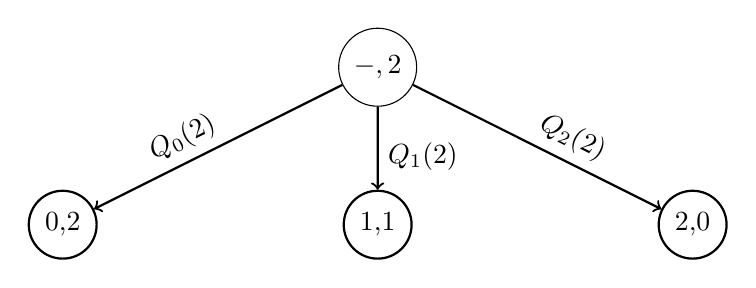
\begin{tikzpicture}[level/.style={->,thick,level distance = 20mm, sibling distance=40mm/#1}]

\node [circle,draw] (z) {$-,2$}
  {child{node [circle,draw] (a) {0,2} edge from parent
            node[ sloped, above, pos=.6] {$Q_{0}(2)$}}
  child {node [circle,draw] (b) {1,1} edge from parent
            node[ right, pos=.6] {$Q_{1}(2)$}}
  child {node [circle,draw] (c) {2,0}{child [grow=up]{node {} edge from parent [draw=none]}} edge from parent
            node[ sloped, above, pos=.6] {$Q_{2}(2)$}}
};
\end{tikzpicture}
\caption{Transaction probabilities to split a set of 2 elements into two sets with $i$, $j$ elements}
\end{figure}

\subsubsection{Example}

\begin{figure}[htbp!]
\centering
\ovalbox{
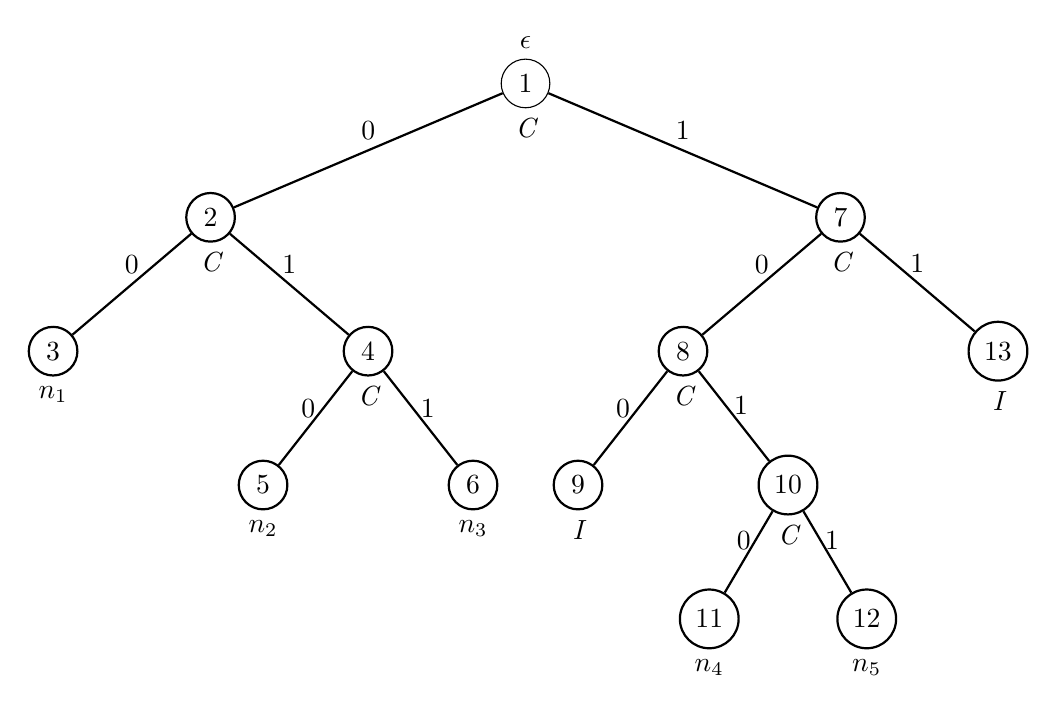
\begin{tikzpicture}[level/.style={thick,level distance = 17mm, sibling distance=80mm/#1}]

\node [circle,draw,label=below:\itshape C,label=above:$\epsilon$] (r){1}{
  	child{node [circle,draw,label=below:\itshape C] {2} {
		child{ node [circle,draw,label=below:$n_{1}$] {3} edge from parent node[ above, pos=.5] {0}
			}
		child{ node [circle,draw, label=below:\itshape C] {4}{		
			child{ node [circle,draw,label=below:$n_{2}$] {5} edge from parent node[ above, pos=.6] {0}}
			child{ node [circle,draw,label=below:$n_{3}$] {6} edge from parent node[ above, pos=.6] {1}}
			} edge from parent node[ above, pos=.5] {1}}
			} edge from parent node[above, pos=.5] {0}
  		}
  	child {node [circle,draw, label=below:\itshape C] {7}{
		child{ node [circle,draw, label=below:\itshape C] {8}{
			child{ node [circle,draw,label=below:\itshape I ] {9} edge from parent node[ above, pos=.6] {0}}
			child{ node [circle,draw,label=below:\itshape C] (s10){10} {
				child{ node [circle,draw,label=below:$n_{4}$] {11} edge from parent node[ above, pos=.6] {0}}
				child{ node [circle,draw,label=below:$n_{5}$] (s12){12} edge from parent node[above, pos=.6]{1} }
			}edge from parent node[ above, pos=.6] {1}}
		} edge from parent node[ above, pos=.5] {0}}
		child{ node [circle,draw,label=below:\itshape I ] {13} edge from parent node[ above, pos=.5] {1}}
		} edge from parentnode[ above, pos=.5] {1}
	}
	
};
\end{tikzpicture}
}
\caption{An istance of the binary tree algorithm for $n=5$ nodes. The number inside the each circle identifies the slot number. The label below identifies the event occurring: \textit{I} for \emph{idle}, \textit{C} for \emph{collision}, $n_{i}$ for resolution of node $i$ }.
\label{example-bbt}
\end{figure}

In figure \ref{example-bbt} we provide an example to further investigate the behavior of the algorithm. We notice that the instance start with a collision in slot 1. Then nodes $n_{1}$, $n_{2}$, $n_{3}$ decide to proceed with a retransmission while $n_{4}$, $n_{5}$ remain idle. In slot 2 we see another collision, after it $n_{1}$ decide to transmit again while $n_{2}$ and $ n_{3}$ to stay quiet. In slot 3 we have the first resolution, $n_{1}$ send successfully its message and won't no more take part to the collision resolution.\\
We notice that we can know the cardinality of a collision only after it has been fully  resolved. For example we know only after slot 6 that the collision in slot 2 involved 3 nodes.\\

\subsubsection{Nodes addresses}

Looking carefully to the tree you can see that each node resolved is characterized by an \emph{address}: the path from the root to node $n_{i}$ gives  a string of bits. For example node $n_{4}$'s address has as prefix 1010. The prefix in this case can be equivalent to the address but, in a more general case, node address can be a longer string. Assuming in fact that node $n_{4}$'s full address is the 8 bit long string 10100010, running the algorithm brings to the discovery of only the first 4 bits since the collision become resolved without requiring further split of the batch and deeper collision tree investigation (collision in level $t$ provokes a split and a deeper investigation in the tree at level $t+1$ and it requires to consider bit $t+1$ of the nodes' addresses).\\

\subsubsection{Tree traversal rules}

The inquirer must provide feedback about the event in a slot but tree walking can be either explicit or implicit. It is explicit if, with feedback, the reader provide also the address in the root of the currently enabled sub-tree. Otherwise it is said to be implicit and each node compute autonomously the new enabled sub-tree.\\
We assume, following the conventional approach, to visit the tree in pre-order, giving precedence to sub-trees starting with 0.\\
Initially all nodes are enabled so the prefix is the empty string $\epsilon$, the root address. $\epsilon$ is considered to be prefix of any string.\\
Let $b_{1..k}$, with $b_{i} \in \{0,1\}$, be the current enabled $k$-bit prefix and \emph{event} $\in \{I,S,C\}$.\\
The possible cases are: \textcolor{red}{qui incasino un po' le cose con una notazione un po' imprecisa}
\begin{enumerate}
\item if \emph{event} is $C$: no matter about $b_{1..k}$, next enabled interval will be $b_{1..k}0$ 
\item if \emph{event} is not $C$ and $b_{k}=0$: we successfully resolved the left part of the sub-tree, now we will look for right one. Next enabled prefix will be $b_{1..k-1}1$
\item if \emph{event} is not $C$ and $b_{k}=1$: we successfully resolved the right part of the sub-tree, now we will look for right one. Let $t = \arg\underset{i \in 1..k}{\max}|b_{i}=0$, in other words the position of the right most 0 in the prefix, if any. The new enabled interval will be $b_{t-1}1$.\\
If $t$ is undefined then in $b_{1..k}$ there is no 0. This means that $b_{1..k} = \epsilon$ or $b_{1..k}=\underbrace{1\dots 1}_{k}$ in both cases this indicates all the three has been explored.\\ So this work also for termination condition.\\
You can see this rule applied after slot 6 and 12 for right branch exploration and 13 for termination.
\end{enumerate}

\subsubsection{\textcolor{red}{Real value approach}}
\textcolor{red}{Decidere se inserire o meno le considerazioni sulla visione degli indirizzi dei nodi come numeri reali tra 0 e 1 e della risoluzione come intervalli reali abilitati contenenti un solo nodo}\\
Every length binary string can be also interpreted as a number in the interval $[0,1)$
\begin{equation*}
11001 \leftrightarrow 1 \cdot 2^{-1} + 1 \cdot 2^{-2} + 0 \cdot 2^{-3} + 0 \cdot 2^{-4} +1 \cdot 2^{-5} 
\end{equation*}
by associating to each position in the string a different power of 2.\\

\subsection{Modified Binary Tree}

Modified binary tree is a simple way to improve the basic variant for the binary tree algorithm.\\ The observation is that, during the tree traversal, sometimes we know in advance if the next slot there will be a collision. This happens when, after a collided slot ($\tau$), we get and idle slot ($\tau+1$) in the left branch of the binary tree: visiting the right branch ($\tau+2$) we will get a collision for sure.\\
In fact in slot ($\tau$) we know that in the sub-tree there are at least 2 nodes and none of them owns to the left-branch sub-tree ($\tau+1$). So they must be in the right sub-tree and when enabled to transmit ($\tau+2$) transmissions will brake.
Solution is to use previous node ($\tau+2$) as a virtual node, to skip it, and continue visiting node ($\tau+1$).$sibling$.$leftchild$ in slot $(\tau+2)$.
This let us save a slot.


\begin{figure}[htbp!]
\centering
\ovalbox{
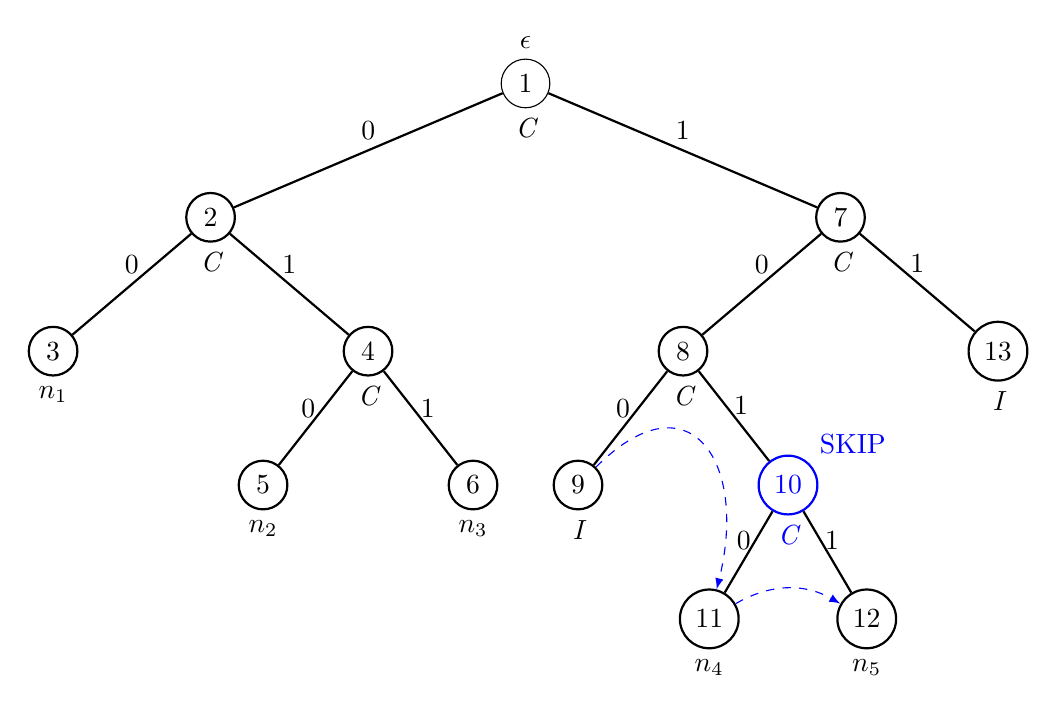
\begin{tikzpicture}[level/.style={thick,level distance = 17mm, sibling distance=80mm/#1}]

\node [circle,draw,label=below:\itshape C,label=above:$\epsilon$] (r){1}{
  	child{node [circle,draw,label=below:\itshape C] {2} {
		child{ node [circle,draw,label=below:$n_{1}$] {3} edge from parent node[ above, pos=.5] {0}
			}
		child{ node [circle,draw, label=below:\itshape C] {4}{		
			child{ node [circle,draw,label=below:$n_{2}$] {5} edge from parent node[ above, pos=.6] {0}}
			child{ node [circle,draw,label=below:$n_{3}$] {6} edge from parent node[ above, pos=.6] {1}}
			} edge from parent node[ above, pos=.5] {1}}
			} edge from parent node[above, pos=.5] {0}
  		}
  	child {node [circle,draw, label=below:\itshape C] {7}{
		child{ node [circle,draw, label=below:\itshape C] (s8) {8}{
			child{ node [circle,draw,label=below:\itshape I ] (s9){9} edge from parent node[ above, pos=.6] (s89){0}}
			child{ node [circle,draw,blue,label=below:\itshape \textcolor{blue}{C},label=45:\textcolor{blue}{SKIP}] (s10){10} {
				child{ node [circle,draw,label=below:$n_{4}$] (s11){11} edge from parent node[ above, pos=.6] (s1011){0}}
				child{ node [circle,draw,label=below:$n_{5}$] (s12){12} edge from parent node[above, pos=.6]{1} }
			}edge from parent node[ above, pos=.6] {1}}
		} edge from parent node[ above, pos=.5] {0}}
		child{ node [circle,draw,label=below:\itshape I ] {13} edge from parent node[ above, pos=.5] {1}}
		} edge from parentnode[ above, pos=.5] {1}
	}
	
};

\draw [-latex,blue,thin,dashed] (s9) .. controls ++(45:2) and ++(0.5,2) .. (s11);
\draw [-latex,blue,thin,dashed] (s11) to [bend left ](s12);
\end{tikzpicture}
}
\caption{Same example as in Figure \ref{example-bbt} but using \algname{MBT}: tree structure remains the same but node 10 is skipped in the traversal}
\label{example-mbt}
\end{figure}

\chapter{Batch Size Estimate Techniques}
We present here some noteworthy techniques for batch size estimate that can be found in literature.
If the technique was not already identified by a name or associated to a acronym we used the name of one authors as reference.
\section{CBT}
non è propriamente di stima ma di risoluzione parziale, cmq può essere usato come alg di stima 
\section{Cidon}
risoluzione di un batch parziale. mapping come in ``Real value approach''
\section{Greenberg}

Greenberg algorithm is simply straightforward.
\algsetup{indent=2em} 
\begin{algorithm}[h!]
\caption{\algname{Greenberg}}
\label{alg-greenberg}
\begin{algorithmic}
\STATE $i\gets 0$
\REPEAT
	\STATE $i\gets i+1$ 
	\STATE choose to transmit with probability $2^{-i}$
\UNTIL {no collision occurs}
\STATE $\hat{n} \gets 2^{i}$
\end{algorithmic}
\end{algorithm}

The idea behind algorithm \ref{alg-greenberg} is quite simple. As the algorithm goes on the initial unknown batch size $n$
comes progressively sliced into smaller pieces. Only the nodes virtually inside the slice are allowed to transmit.\\
If two o more nodes decide to transmit we get a collision,\\
An important note is that the algorithm always involve all the nodes in the batch: in each stage of the algorithm each node has to take a choice if transmit or not. 
Each choice is independent of what the nodes did in the previous steps. 



\begin{figure}[t]
    
    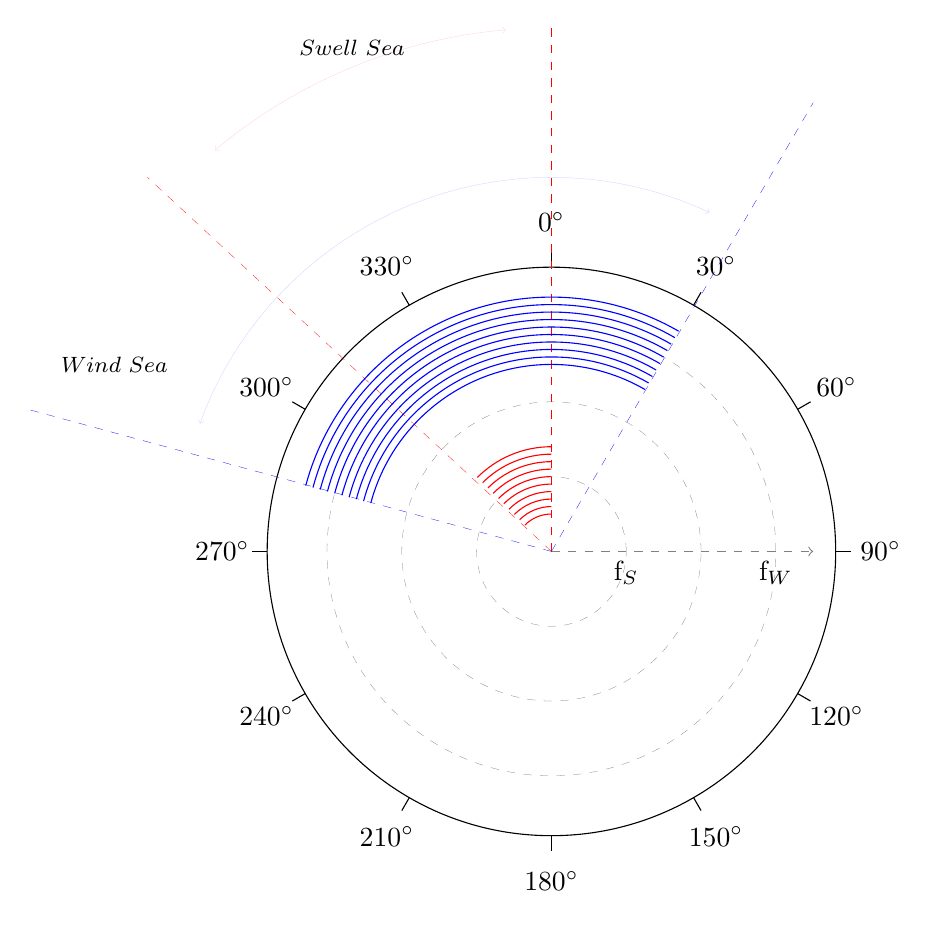
\begin{tikzpicture}[scale=.95]  
        \draw (0, 0) circle (3.8cm);
        \foreach \x  in {0, 30, ..., 330}
        \draw (-\x+90:3.8) -- (-\x+90:4.0) (-\x+90:4.4) node {$\x^\circ$};
        \foreach \x  in {0,1, ..., 3}
        \draw[dashed,ultra thin,gray] (0,0)circle(\x);
        \draw[->,dashed,gray](0,0) to[] (3.5,0);
        %Add labels with names of the primary and secondary colors.
        \foreach \x/\text in {1/f$_{S}$, 3/f$_{W}$}
        \draw (\x,0) node [below]{\text};
        \foreach \x/\text in {.5,.6,...,1.5}
        \draw [-,thin,red] (90:\x) arc(90:135:\x);
        \draw[-,ultra thin,red,dashed] (0,0) to[] (0,7);
        \draw[-,ultra thin,red,dashed] (0,0) to[] (-5.4,5);
        \foreach \x/\text in {2.5,2.6,...,3.5}
        \draw [-,thin,blue] (60:\x) arc(60:165:\x); 
        \draw[-,ultra thin,blue,dashed] (0,0) to[] (3.5,6);
        \draw[-,ultra thin,blue,dashed] (0,0) to[] (-7,1.9);
            
        \draw [<->,ultra thin,blue!20] (65:5) arc(65:160:5);
        \draw [<->,ultra thin,red!20] (95:7) arc(95:130:7);
        \path[font=\footnotesize]
        (-3.5,6.5) node[above right] {$Swell\ Sea$}
        (-5,2.5) node[left] {$Wind\ Sea$};
        %(.5,0) node[above right] {$0.1\ Hz$}
        %   (3.8,.2) node[left] {$0.3\ Hz$};
        %   
    
    \end{tikzpicture}
    \caption[Idealised directional spectrum]{Immagine provvisoria da usare come base di partenza}
    \label{fig:sp2d}
\end{figure}

\section{Window Based}
\chapter{Inital Batch size estimate}
\chapter{Comparison}

\begin{thebibliography}{99}
 
\bibitem{popovski}
  Peter Popovski, Frank H.P. Fitzek, Ramjee Prasad, \emph{ A Class of Algorithms for Collision Resolution with Multiplicity Estimation}, Springer, Algorithmica, Vol. 49, No. 4, December 2007, 286-317
  
\bibitem{lucent}
Murali Kodialam, Thyaga Nandagopal, \emph{Fast and Reliable Estimation Schemes in RFID Systems}, MobiCom '06: Proceedings of the 12th annual international conference on Mobile computing and networking, ACM , September 2006, 322-333 
 
\bibitem{cidon}
 Israel Cidon, Moshe Side, \emph{Conflict Multiplicity Estimation and Batch Resolution Algorithms}, IEEE Transactions On Information Theory, Vol. 34, No. 1, January 1988, 101-110
 
\bibitem{greenberg87}
  Albert G. Greenberg, Philippe Flajolet,  Richard E. Ladner,
  \emph{Estimating the Multiplicities of Conflicts to Speed Their Resolution in Multiple Access Channels},
  Journal of the Association for Computing Machinery,
  Vol 34, No. 2, April 1987, 289-325
  
 \bibitem{capetanakis}
  J.I. Capetanakis, \emph{ Tree algorithms for packet broadcast channels}, IEEE Transactions On Information Theory, Vol. 25, No. 5, September 1979, 505-515
 \end{thebibliography}
\end{document}